\chapter{The human spine}
\par{
    This document presents a model for automatic segmentation of \acrfull{ct} and \acrfull{mri} images of the lumbar spine.
    This chapter introduces these terms\footnote{This work is not a medical desideration. For in-depth knowledge on the anatomy and physiology of the spine, consult the specialized literature.}.
    Secondly, it gives a basic overview of the medical imaging techniques. 
    Finally, it touches upon a specific medical procedure in which this information is used: the minimally invasive surgery of a spinal hernia.
}



\section{Anatomy of the human spine}

\todo[inline]{Assure all citations are ok.}
\par{
    The spinal column, vertebral column or backbone \footnote{NL: \textit{wervelkolom}} is a structure of 34 bones. 
    It holds the body upright while providing it with the mobility to bend and twist.
    the \textit{intervertebral discs} make this possible. These consist of a ring of fibrocartilage and an inner gel-like centre and form an articulation between two vertebrae.
    Moreover, the vertebral column serves as a conduit for major nerves running from the brain to the toes.
    The spinal column, as illustrated in figure \ref{fig:spineimage} can be divided into five regions:
}

\begin{description}
    \item[the Cervical spine:] 7 vertebrae of the neck, indicated by C$_1$ to C$_7$\footnote{Vertebrae are numbered from the head down. C1 (\textit{atlas}) is the vertebra closest to the head}.
    \item[the Thoracic spine:] 12 vertebrae of the middle back (T$_1$ to T$_{12}$).
    \item[the Lumbar spine:] 5 vertebrae that form the lower back. These are commonly referenced as L$_1$ to L$_5$.
    \item[the Sacrum:]\footnote{NL: \textit{Heiligbeen}} This is a structure consisting of 5 naturally fused vertebrae (S$_1$-S$_5$).
    \item[the Coccyx:]\footnote{NL: \textit{Stuit of staartbeen}} Structure of 3 to 5 naturally fused vertebrae at the end of the spinal column.
\end{description}


\begin{SCfigure}[][h!]
    \centering
    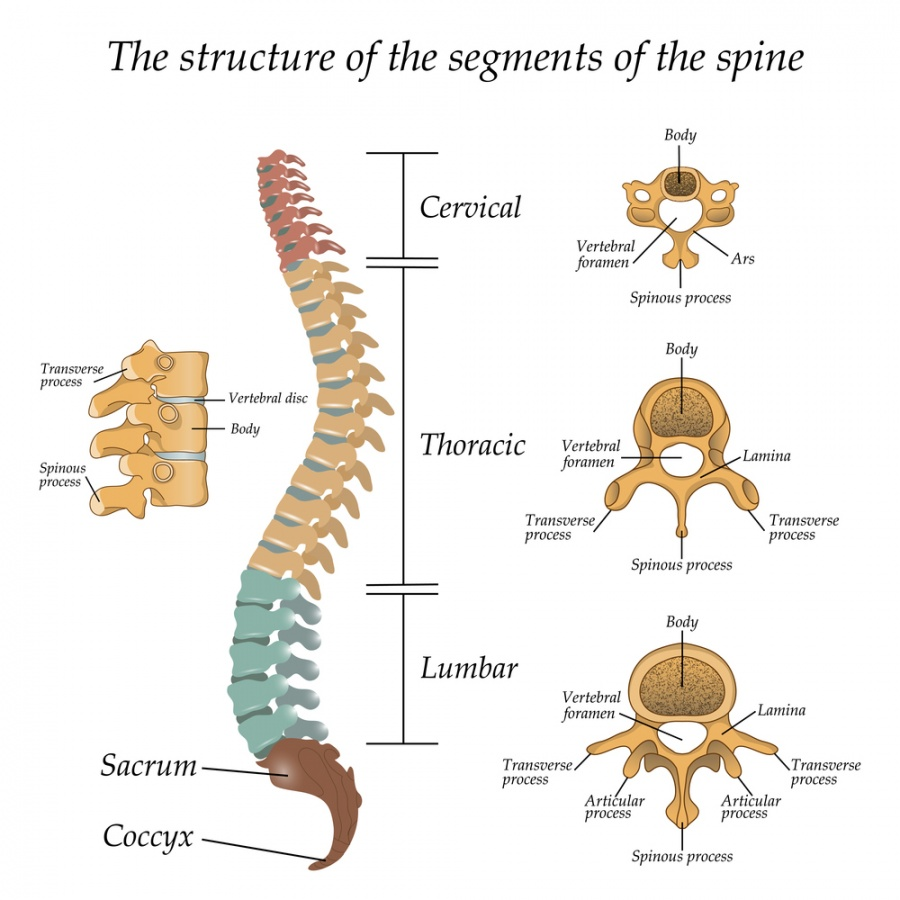
\includegraphics[width=10cm]{/home/thesis/images/SpineModel.jpeg}
    \caption{\label{fig:spineimage}Model of the human spine. The five vertebrae in green form the lumbar spine. They are referred to as \textit{L1} to \textit{L5} from top to bottom. }
\end{SCfigure}

\section{Pathologies of the human spine}
\par{
    This document does not aim to provide an exhaustive list of all human spinal pathologies. 
    Two pathologies are interesting to discuss further as an introduction to this work since they occur in the data used in this project, see page \pageref{sec:datasets} for further details.
}
\par{
    First, there is \textit{scoliosis}, which is a sideways curve of the spine.
    The severity of this condition can vary from relatively mild to severe. 
    In severe cases, scoliosis can affect the patient's movement and breathing.
    \todo[inline]{image}.
}
\par{
    Second, there is the \textit{spinal hernia} or spinal disc herniation\footnote{Spinal disc herniation is sometimes referred to as a \textit{slipped disc}.}. 
    A spinal hernia is caused by damage to the \textit{annulus fibrosus}\footnote{The fibrocartilage ring around the softer gel-like centre of the intervertebral disc.}. 
    This damage can cause the intervertebral disc to bulge out. 
    This condition is painful due to the inflammation reaction, and in severe cases, the bulging material can irritate or cause impingement of the critical nerves along the spine.
    The nerve impingement can even lead to radiating pain to the limbs or even limb paralysis.
    In severe cases, a spinal hernia requires surgical treatment.
    This specialized procedure requires repeated medical imaging to allow the surgeon to investigate the situation before the operation accurately and assure correct positioning of the instruments during the intervention.
}

\section{Medical imaging of the human spine\label{sec:medical_imaging}}
\marginpar{
        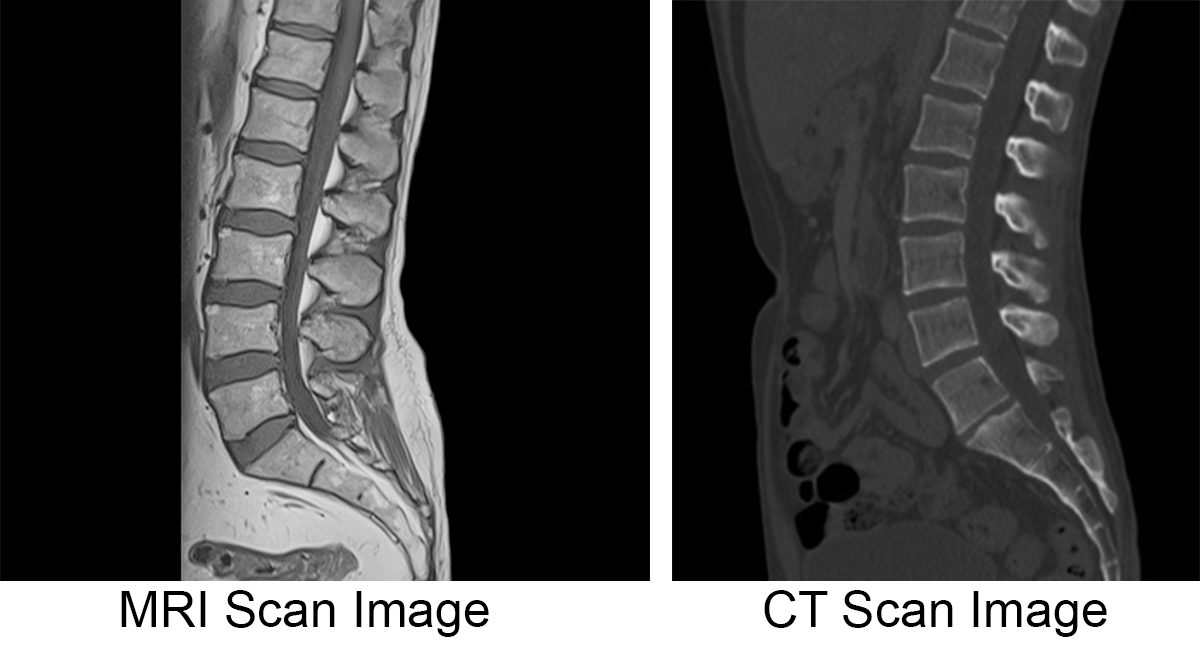
\includegraphics[width=5cm]{/home/thesis/images/MRI_CT_images.jpeg}
        \captionof{figure}{Illustration of \acrshort{ct} and \acrshort{mri} images of a human lumbar spine.}
        \label{fig:mri_ct}
    }

\todo[inline]{Describe Hounsfield scale.}

\par{
    For spinal pathology diagnosis of the \hlnote{main}{Is this correct? Find reference.} medical imaging techniques are \acrfull{ct}, \acrfull{us} and \acrfull{mri}. 
    These techniques allow non-invasive visualization of the spine and discs in three dimensions.
    Slices from these volumetric scans are illustrated in \ref{fig:mri_ct}.
}

\subsection{CT scan}
\par{
    The \acrfull{ct}\footnote{Also known as CAT-scan, for Computed Axial Tomography or Computer-assisted Tomography.} is a non-invasive medical imaging procedure
    \footnote{CT scans are primarily used for medical purposes. 
    It is also used in industry for non-destructive component and assembly inspection.
    In geology, it is used to identify materials in a drill core quickly. In archaeology, it is used for the non-destructive investigation of artefacts. } 
    for diagnostic purposes. 
    A \acrlong{ct} procedure consists of the combination of an array of X-ray attenuation images taken with a \hlnote{rotating X-ray tube}{Add illustration}. 
    These images can be combined with a tomography algorithm to reconstruct a volumetric representation of the radiographic density.
}
\par{
    \acrshort{ct} is a versatile technique with various medical diagnostic applications. 
    Contrary to \acrfull{mri} imaging, this technique is suitable for patients with a pacemaker or insulin pump since there are no magnetic fields involved.
    The main disadvantage of \acrshort{ct} is the exposure to ionizing radiation of the patient and the risk of exposure of the medical professional to the same radiation.
    The image quality increases with radiation dose, but so does the probability of radiation-induced cancer.
    Improvement of the reconstruction algorithms to obtain higher-resolution images without reducing the radiation dose is an ongoing area of research. 
}

\subsection{MRI scan}
\par{
    The \acrfull{mri} scan is a medical imaging technique that is not based on ionizing radiation\footnote{Eventhough the alternative name \textit{nuclear} magnetic resonance (NMR) might confuse.}.
    \acrshort{mri} imaging will visualize the concentration of hydrogen\footnote{In theory, other atoms than hydrogen can be excited by adapting the excitation frequency. This is rarely done.} atoms.
    The patient is positioned in a tunnel where a high (up to several Tesla) constant magnetic field is applied. A temporary oscillating signal is applied with the resonance frequency corresponding to hydrogen atoms is superposed on the static magnetic field.
    The hydrogen atoms will fall back to the equilibrium state, emitting radiofrequency (RF) signals. These can be measured by receiving coils.
    After excitation, the hydrogen in the water atoms in the patient's body tissues returns to the equilibrium state. \acrlong{mri} is particularly suitable for visualization of tissue with higher water content, such as tumours and infections, and to visualize fat.
}
\par{
    An \acrshort{mri} scan can be \textit{T1 weighted} or \textit{T2 weighted}. 
    The difference between these two techniques lies in whether the image is constructed based on the relaxation time of the magnetization is colinear with the direction of the static field (T1) or the magnetization perpendicular to the static field (T2).
    While areas with higher water content, such as infected areas, will release a higher signal on a T2-weighted \acrshort{mri} scan, the same images will show a lower signal strength for T1-weighted scans.
    The use of these different techniques of \acrshort{mri} scans is application-dependent.  
}
\par{
    Contrary to \acrfull{ct} scans, the \acrlong{mri} procedure does not expose the patient of radiation. Due to the high magnetic fields, the technology cannot be used for patients with pacemakers, cochlear implants or other metallic objects in the body.
    \acrshort{mri} allows to visualize soft tissue better than \acrshort{ct} images. An \acrshort{mri} image allows visualizing both the grey and white brain matter, while this is not possible with \acrshort{ct} images.
    Although both techniques produce images that resemble each other, none of both techniques can replace the other one completely.
}

